\section{Opérateurs de flux}
L'avantage de la gestion de flux est de pouvoir gérer la dynamique des données via des opérateurs dédiés. Astral est construite sur la sémantique a deux concepts, il nous faut donc définir les opérateurs flux vers relation (fenêtres) et relation vers flux (streamers). Puis, nous définirons et explorerons des opérateurs spécifiques à la gestion de flux étant : la gestion des modifications des relations et des \textit{batchs}.
\subsection{Fenêtres}
L'opérateur de fenêtre est un des opérateurs les plus étudiés dans la littérature. Toutefois, son comportement est encore flou sur certains points. La formalisation de son fonctionnement permettra donc une meilleure compréhension.
\subsubsection{Association position-\textit{batch}}
Avant de définir formellement l'opération de fenêtrage, nous avons besoin d'un outil pour gérer l'association entre la position d'un n-uplet et de son \textit{batch}. La fonction $\tau_S$ définit cette association. 
\begin{defi}[Fonction position-\textit{batch}]\label{def:tau}
    Soit $S$ un flux,

    La fonction $\tau_S : \N\cup\{-1\}\to \TN$ est la fonction associant un entier à l'identifiant de \textit{batch} du seul n-uplet présent à cette position.

    Par convention, $\tau_S(-1)=(t_0,0)$.
\end{defi}

Par corollaire de l'hypothèse fondamentale~\ref{hyp:ordres}, la fonction $\tau_S$ est donc croissante non-stricte. Ainsi, il est possible de définir une pseudo inverse $\rtau_S$ capable de donner une position (la maximale en l'occurence) pour un \textit{batch} donné.
\begin{coro}[Fonction pseudo-inverse $\tau$]
    Soit $S$ un flux,

    La pseudo-inverse $\rtau_S:\TN\to \N\cup\{-1\}$ existe et correspond à la plus grande position du \textit{batch} donné en entrée. Si aucun \textit{batch} n'existe, le plus proche est utilisé. Formellement, $$\forall b \in \TN, \qquad \tau_S^{-1}(b) = \sum_{n=-1}^{+\infty} n \indic_{[\tau_S(n),\tau_S(n+1)[}(b)$$
\end{coro}

De par sa nature, la fonction $\tau$ et sa pseudo-inverse partagent des propriétés intéressantes que nous pourrons réutiliser lors de démonstrations formelles.
\begin{prop}[Propriétés de $\tau$]
    Soit $S$ un flux, alors les propriétés suivantes sont correctes :
    \begin{eqnarray*}
        t_0 & \leq & \tau_S(0) \\
        \tau_S(\tau_S^{-1}(b)) & \leq & b \\
        n & \leq & \tau_S^{-1}(\tau_S(n))
    \end{eqnarray*}

    De plus, si $\exists s \in S$, $\BS(s)=b$, alors $\tau_S(\tau_S^{-1}(b)) = b$.
\end{prop}
\subsubsection{Description de séquences de fenêtres}
Afin de se rapproche le plus possible d'un aspect déclaratif, nous souhaitons décorréler l'opérateur de fenêtre en deux objets mathématiques : la description et l'opérateur exécutable. Ce dernier prendra une description en argument pour pouvoir représenter la relation temporelle résultante. Le principe des descriptions de séquences de fenêtres est assez simples, il suffit de décrire deux bornes évoluant de manière discrête, et un taux d'évaluation de ces bornes.

\begin{defi}[Description de Séquence de Fenêtre (DSF)]
    Soient $\D$ et $\D'$ pouvant être $\T$ ou $\N$, une description de séquence de fenêtre (DSF) est un triplet $(\alpha,\beta,r)$ tel que :
\begin{itemize}
    \item $r \in \D$ est le taux d'évaluation des bornes de la fenêtre
    \item $\alpha$ et $\beta$ sont deux fonction de $\N\to D'$ représentant l'évolution des bornes.
\end{itemize}

$\alpha(j)$ et $\alpha(j)$ définissent les $j\eme$ valeures des bornes. La première étant donnée pour $j=0$. Ces fonctions se doivent de vérifier les propriétés suivantes (en considérant $\D=\D'=\T$) :
$$\forall j \in \N, \begin{cases} \alpha(j) \leq \beta(j) & \textrm{le début est avant la fin}\\ \alpha(j) \geq t_0 & \textrm{le début existe} \\ \beta(j) \leq jr + \beta(0) & \textrm{la fin est accessible} \end{cases}$$
    Les conditions pour les autres cas pour $\D$ et $\D'$ sont évidentes par application des fonctions $\tau_S$ et $\tau_S^{-1}$.
\end{defi}

\begin{example}
    Nous souhaitons relever tous les $100$ relevés de charge processeur, les $10$ derniers relevés. Dans ce cas, nous souhaitons obtenir une séquence de fenêtres positionnelles générées tous les $100$ n-uplets ($r=100\in \N$). Nous appliquons des bornes positionnelles donc $\alpha,\beta \in (\N\to\N)^2$. La première fenêtre couvrira du $91\eme$ n-uplet au $100\eme$. Ainsi : $\alpha(0) = 91$ et $\beta(0) = 100$. L'évolution des bornes étant linéaire, nous avons donc :
\begin{eqnarray*}
 \alpha(j) &=& 100j+91\\
 \beta(j) &=& 100j + 100\\
 r & = & 100
\end{eqnarray*}
\end{example}

La création de fenêtre nécessite l'association entre les n-uplets du flux et le numéro de fenêtre décrit dans la \textit{DSF}. Pour cela, nous utilisons une \textit{fonction d'attente} utilisant les identifiants de \textit{batch}. Cette fonction donne le rang de la dernière fenêtre au moment indiqué par le batch. Le terme \textit{attente} est lié au fait que l'évaluateur devra attendre avant le prochain changement de $\gamma$.
Nous retrouvons dans cette fonction le caractère \textit{bloquant} des fenêtres.
\begin{defi}[Fonction d'attente $\gamma$]
    Soit $S$ un flux, soit $(\alpha,\beta,r)$ une DSF,

    La fonction d'attente de la DSF est une fonction $\TN \to \N$ associant un identifiant de \textit{batch} à l'identifiant de la dernière fenêtre complétée.
\begin{itemize}
 \item  Si $r\in\T$, cette fonction est définie par $\gamma : (t,i) \mapsto \left\lfloor \frac{t-\beta(0)}{r} \right\rfloor$.
 \item  Si $r\in\N$, cette fonction est définie par $\gamma : (t,i) \mapsto \left\lfloor \frac{\rtau_S(t,i)-\beta(0)}{r} \right\rfloor$.
\end{itemize}
\end{defi}
\begin{example}
    En reprenant l'exemple précédent, après simplification nous obtenons : $$\gamma(b) = \left\lfloor \frac{\rtau_S(b)}{100}\right\rfloor-1.$$
    Si nous supposons que le flux produit un n-uplet par seconde (ainsi, $\rtau_S(t,i) = \lfloor t/1s \rfloor$) : alors $\gamma(1024s,0) = \left\lfloor \frac{1024}{100}\right\rfloor-1 = 9$. Nous avons donc bien la $10\eme$ fenêtre ($j=9$) comme la dernière fenêtre créée à ce moment.
\end{example}

\subsubsection{L'opérateur}
Il devient désormais possible de définir un opérateur permettant  de générer une relation temporelle à partir d'un flux donné. Cette relation temporelle gère ses changements d'état grâce à la fonction $\gamma$. De manière générale, une DSF peut être ramenée simplement à une expression plus générale $(\alpha,\beta,\gamma)$ ce que nous utiliserons pour la définition de séquence de fenêtres.
\begin{defi}[Opérateur de Séquence de Fenêtres]
	Soit $S$ un flux et $(\alpha, \beta, \gamma)$ une description de séquence,
	
	L'opérateur de séquence de fenêtres est défini par : $\forall b \in \TN$, 
	\begin{itemize}
		\item Si $\gamma(b) \geq 0$, 
		\begin{itemize}
			\item Si la description possède des bornes temporelles :
			$$S[\alpha,\beta,\gamma](b) = \left\{s\in S, \ (\alpha(\gamma(b)),0)\leq \BS(s) \leq (\beta(\gamma(b)),i)\right\}$$
			\item Si la description possède des bornes positions :
			$$E(b) = \left\{s\in S, \ \tau_S(\alpha(\gamma(b)))\leq \BS(s) \leq \tau_S(\beta(\gamma(b)))\right\}$$
			$$S[\alpha,\beta,\gamma](b) = \{s \in E(b) / (\#E(b) - \pos_{E(b)}(s)) \leq \beta(\gamma(b)) - \alpha(\gamma(b))$$
		\end{itemize}
		\item Si $\gamma(b) <0$ alors $S[\alpha,\beta,\gamma](b) = \emptyset$
	\end{itemize}
\end{defi}

Plusieurs remarques peuvent être formulées sur cette définition. Tout d'abord, les expressions sont différentes si les bornes sont positionnelles ou temporelles. Pour les fenêtres temporelles, l'opérateur inclue les n-uplets dont l'identifiant de \textit{batch} s'étend :
\begin{itemize}
	\item[\textbf{depuis}] le premier \textit{batch} de la fenêtre : $(\alpha(\gamma(t,i)),0)$, i.e. ceux dont le \textit{timestamp} est supérieur à la borne inférieur.
	\item[\textbf{jusqu'au}] dernier \textit{batch} de la fenêtre : $(\beta(\gamma(t,i)),i)$. Ce qui correspond au $i\eme$ \textit{batch} ayant le \textit{timestamp} inférieur ou égal à la borne.
\end{itemize}
Il est important de voir que $S[\alpha,\beta,\gamma]$ pourra changer à l'arrivée d'un nouveau \textit{batch}, même si le \textit{timestamp} ne change pas. Ne pas inclure ces modifications ferait perdre des données de dynamicités à la fenêtre. Nous retrouvons donc les problématiques explorées dans la section~\ref{sec:rw:sgfd:modeles}.

Pour les fenêtres positionnelles, la gestion est plus délicate. Si nous considérons que le flux réparti ses \textit{batchs} (donc un n-uplet par \textit{batch}), alors $E(b) = S[\alpha,\beta,\gamma](b)$. Mais dans le cadre général, $E(b)$ contient l'ensemble des n-uplets potentiels et la séquence $S[\alpha,\beta,\gamma](b)$ en est un sous-ensemble dont la taille est exactement celle décrite dans la DSF (sélections des n-uplets les plus récents). De plus, nous remarquons que $\gamma$ en positionnel est dirigé par $\rtau_S$ qui fournit la position maximale en cas d'égalité de \textit{batch}, ce qui nous garanti de couvrir l'ensemble des n-uplets concernés.

	
\begin{example}
	La figure~\ref{fig:contrib:astral:fenetres} montre l'évolution d'une séquence où la fenêtre glisse de $2$ secondes toutes les $2$ secondes ($r=2$) avec une taille constante de $3$ secondes. $t_0 = 0$ par simplicité ici. 
La première fenêtre possède les bornes $\alpha(0) = t_0+ 0s$ et $\beta(0) =t_0+3s$. Le glissement étant de $2s$ la description de fenêtre est donc $$\forall j \in \N, \begin{cases} \alpha(j)  & =\ i*2s+t_0 \\ \beta(j) & = \ j*2s+3s+t_0\end{cases}$$
La relation temporelle généré par cette DSF peut être noté $S[2js,2js+3s,2s]$.  Le calcul de son état à un instant est simple. Prenons le batch $(t_0+5.5s,0)$. La fenêtre a calculer est la fenêtre numérotée $\gamma(t_0+5.5s,0) = \left\lfloor \frac{t_0+5.5s-\beta(0)}{r}\right\rfloor = 1$. Ainsi : $S[2js,2js+3s,2s](t_0+5.5s,0) = F_1 = \{s_4,s_5,s_6,s_7,s_8\}$.
\end{example}
\begin{figure}[ht]
	\centering
	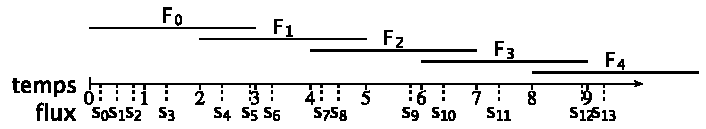
\includegraphics[width=0.7\textwidth]{contrib-astral-fenetres}
	\caption{Séquence de fenêtre de taille $3s$ glissante de $2s$}\label{fig:contrib:astral:fenetres}
\end{figure}

\subsubsection{Fenêtres partitionnées}
L'opérateur de fenêtres partitionnée est très utilisé pour appliquer la même séquences de fenêtres à des sous-flux. Les opérateurs partitionnés sont tous décrit de la même manière. Le principe, illustré dans la figure~\ref{fig:contrib:astral:partition} est de divisé le flux suivant un (ou des) attributs $A$ donné. Sur chacun de ces sous-flux est appliqué un opérateur quelconque. Par la suite, une union est appliquée.
\begin{figure}[ht]
	\centering
	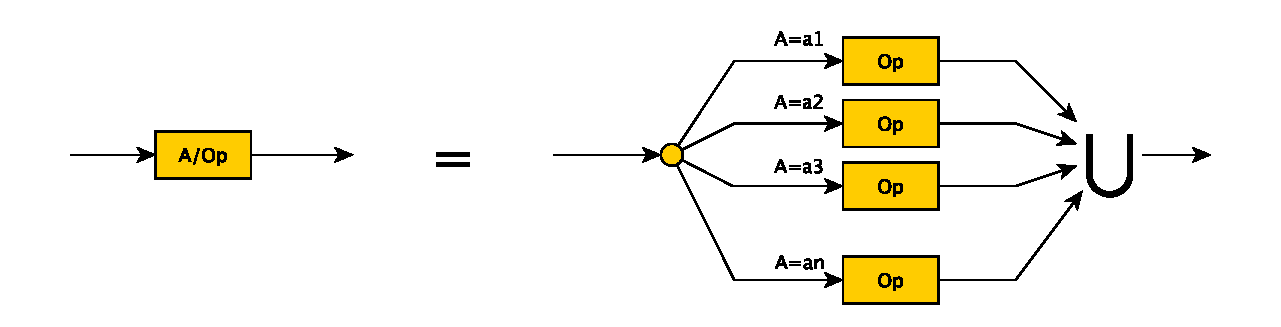
\includegraphics[width=0.9\textwidth]{contrib-astral-partition}
	\caption{Principe d'un opérateur partitionné}\label{fig:contrib:astral:partition}
\end{figure}
\begin{defi}[Séquence de fenêtre partitionnée]
	Soient $S$ un flux, $a_1,...,a_k$ un ensemble d'attributs du schéma de $S$, et $(\alpha,\beta,\gamma)$ une DSF,
	
	Soit $\cup^*$ l'union relationnelle conservatrice des identifiants physiques, 

	Alors la séquence de fenêtre $(\alpha,\beta,\gamma)$ partitionnée par $a_1,...,a_k$ est définie par :
	$$S[a_1...a_k/\alpha,\beta,\gamma] = \mathop{\bigcup\null^*}_{a\in Dom(a_1,...,a_k)} (\sigma_{(a_1,...,a_k)=a} S)[\alpha,\beta,\gamma]$$
\end{defi}

Nous remarquons que nous utilisons la définition conservatrice de l'union relationnelle présenté dans la section précédente, ainsi l'ordre naturel décrit dans le flux d'entrée pourra être retrouvé dans la relation de sortie.
\begin{example}
	L'exemple le plus courant étant la représentation de l'état actuel d'un système à partir d'un flux. Supposons un flux d'entrée $DeviceCPU(deviceId,cpu,\t)$, nous donnant les relevés de charge de processeur. Soit la description de fenêtre rapportant le dernier n-uplet d'un flux : $(1j,1j,1)$. Nous pouvons obtenir la relation temporelle représentant pour chaque dispositif $deviceId$, la dernière valeure connue de $cpu$ et son \textit{timestamp de mesure} $\tau$ : $$DeviceCPU[id/1j,1j,1]$$

	Cet exemple illustre comment nous pouvons passer d'un flux brut à une représentation (dynamique) d'un \textbf{contexte}.
\end{example}

Par la suite, nous utiliserons plusieurs notations simplifiés pour désigner des descriptions de fenêtres courantes décrites dans le tableau~\ref{tab:windows}.
\begin{table}
\centering
\begin{tabular}{c||p{0.4\textwidth}|p{0.4\textwidth}}
  & Définition & Équivalence \\ \bottomrule
 $[L]$ & $[j,j,1]$ &  \\ 
 & \multicolumn{2}{p{0.8\textwidth}}{La séquence de fenêtre où chaque fenêtre ne contient que le dernier n-uplet du flux. Cette séquence est égale à $[B]$ si le flux réparti ses n-uplets avec un n-uplet par \textit{batch}.} \\ \hline
 $[B]$ & $[\tau_S^{-1}(\tau_S(j)^-)+1,j,1]$ & $\{s\in S, \BS(s) = \tau_S\circ\tau_S^{-1}(b)\}$ \\ 
 & \multicolumn{2}{p{0.8\textwidth}}{Séquence de fenêtre où chaque fenêtre contenient le dernier \textit{batch}.} \\\hline
 $[\infty]$ & $[0,j,1]$ & $\{s\in S, \BS(s) \leq b\}$ \\
 & \multicolumn{2}{p{0.8\textwidth}}{Séquence accumulative contenant tout le flux jusqu'au \textit{batch} courant.} \\\hline
 $[T\ r]$ & $[\max(rj-r+t_0,t_0),rj+t_0,r]$ &  \\
 & \multicolumn{2}{p{0.8\textwidth}}{Fenêtre temporelle de taille $r$ se déplaçant toutes les $r$ unités de temps.} \\\hline
 $[P\ r]$ & $[\max(rj-r,0),rj,r]$ &  \\
 & \multicolumn{2}{p{0.8\textwidth}}{Fenêtre positionnelle de taille $r$ n-uplets se déplaçant tous les $r$ n-uplets.} \\
 \toprule
\end{tabular}
\caption{Liste des fenêtres courantes} \label{tab:windows}
\end{table}

Il est important de noter que les équivalences citées sont toutefois non triviales, des démonstrations formelles sont fournies en annexes.

\subsection{Streamers}
\subsection{Domaine}
\subsection{Spread}